\documentclass[../main.tex]{subfiles}

\begin{document}

One of the topics in the A Level Further Maths course is linear transformations, as represented by matrices. This is a topic all about how vectors move and get transformed in the plane. It's a topic that lends itself exceedingly well to visualization, but students often find it hard to visualize this themselves, and there is a considerable lack of good tools to provide visual intuition on the subject. There is the YouTube series \textit{Essence of Linear Algebra} by 3blue1brown\cite{essence-of-linear-algebra}, which is excellent, but I couldn't find any good interactive visualizations.

My solution is to develop a desktop application that will allow the user to define 2x2 matrices and view these matrices and compositions thereof as linear transformations of a 2D plane. This will give students a way to get to grips with linear transformations in a more hands-on way, and will give teachers the ability to easily and visually show concepts like determinants and invariant lines.

\subsection{Computational Approach}

This solution is particularly well suited to a computational approach since it is entirely focussed on visualizing transformations, which require complex mathematics to properly display. It will also have lots of settings to allow the user to configure aspects of the visualization. As previously mentioned, visualizing transformations in one's own head is difficult, so a piece of software to do it would be very valuable to teachers and learners, but current solutions are considerably lacking.

My solution will make use of abstraction by allowing the user to define a set of matrices which they can use in expressions. This allows them to use a matrix multiple times and they don't have to keep track of any of the numbers. All the actual processing and mathematics happens behind the scenes and the user never has to worry about it; they just compose their defined matrices into transformations. This abstraction allows the user to focus on exploring the transformations themselves without having to do any actual computations. This will make learning the subject much easier, as they will able to gain a visual intuition for linear transformations without worrying about computation until after they've built up that intuition.

I will also employ decomposition and modularization by breaking the project down into many smaller parts, such as one module to keep track of defined matrices, one module to validate and parse matrix expressions, one module for the main GUI, as well as sub-modules for the widgets and dialog boxes, etc. This decomposition allows for simpler project design, easier code maintenance (since module coupling is kept to a minimum, so bugs are isolated in their modules), inheritance of classes to reduce code repetition, and unit testing to inform development. I also intend this unit testing to be automated using GitHub Actions.

Selection will also be used widely in the application. The GUI will provide many settings for visualization, and these settings will need to be checked when rendering the transformation. For example, the user will have the option to render the determinant, so I will need to check this setting on every render cycle and only render the determinant parallelogram if the user has enabled that option. The app will have many options for visualization, which will be useful in learning, but if all these options were being rendered at the same time, then there would be too much information for the user to properly process, so I will let the user configure these display options to their liking and only render the things they want to be rendered.

Validation will also be prevalent because the matrix expressions will need to follow a strict format, which will be validated. The buttons to render and animate the matrix will only be clickable when the given expression is valid, so I will need to check this and update the buttons every time the text in the text box is changed. I will also need to parse matrix expressions so that I can evaluate them properly. All this validation ensures that crashes due to malformed input are practically impossible, and makes the user's life easier since they don't need to worry about if their input is in the right format - the app will tell them.

I will also make use of iteration, primarily in animation. I will have to re-calculate positions and values to render everything for every frame of the animation and this will likely be done with a simple \texttt{for} loop. A \texttt{for} loop will allow me to just loop over every frame and use the counter variable as a way to measure how far through the animation we are on each frame. This is preferable to a \texttt{while} loop, since that would require me to keep track of which frame we're on with a separate variable.

Finally, the core of the application is visualization, so that will definitely be used a lot. I will have to calculate positions of points and lines based on given matrices, and when animating, I will also have to calculate these matrices based on the current frame. Then I will have to use the rendering capabilities of the GUI framework that I choose to render these calculated points and lines onto a widget, which will form the viewport of the main GUI. I may also have to convert between coordinate systems. I will have the origin in the middle with positive $x$ going to the right and positive $y$ going up, but I may need to convert that to standard computer graphics coordinates with the origin in the top left, positive $x$ going to the right, and positive $y$ going down. This visualization of linear transformations is the core component of the app and is the primary feature, so it is incredibly important.

\subsection{Stakeholders}

Stakeholders for my app include A Level Further Maths students and teachers, who learn and teach linear transformations respectively. They will be able to provide useful input as to what they would like to see in the app, and they can provide feedback on what they like and what I can add or improve. I already know from experience that linear transformations are tricky to visualize and a computer-based visualization would be useful. My stakeholders agreed with this. Many teachers said that a desktop app that could render and animate linear transformations would be useful in a classroom environment and students said that it would be helpful to have something that they could play around with at home and use to get to grips with matrices and linear transformations.

Some teachers also suggested that it would be useful to have an option to save and load sets of matrices. This would allow them to have a single save file containing some matrices, and then just load this file to use for demonstrations in the classroom. This would probably be quite easy to implement. I could just wrap all the relevant information into one object and use Python's \texttt{pickle} module to save the binary data to a file, and then load this data back into the app in a similar way.

My stakeholders agreed that being able to see incremental animation - where, for example, we apply matrix $\mathbf{A}$ to the current scene, pause, and then apply matrix $\mathbf{B}$ - would be beneficial. This would be a good demonstration of matrix multiplication being non-commutative. $\mathbf{AB}$ is not always equal to $\mathbf{BA}$. Being able to see this in terms of animating linear transformations would be good for learning.

They also agreed that a tutorial on using the software would be useful, so I plan to implement this through an online written tutorial hosted with GitHub Pages, and perhaps a video tutorial as well. This would make the app much easier to use for people who have never seen it before. It wouldn't be a lesson on the maths itself, just a guide on how to use the software.

\subsection{Research on existing solutions}

There are actually quite a few web apps designed to help visualize 2D linear transformations but many of them are hard to use and lacking many features. Arguably the best app that I found was an MIT \enquote{Mathlet} - a simple web app designed to help visualize a maths concept. This one is called \enquote{Matrix Vector}\cite{mit-mathlet-matrix-vector} and allows the user to drag an input vector around the plane and see the corresponding output vector, transformed by a matrix that the user can define, although this definition is finicky since it involves sliders rather than keyboard input.

\begin{figure}[h]
	\centering
	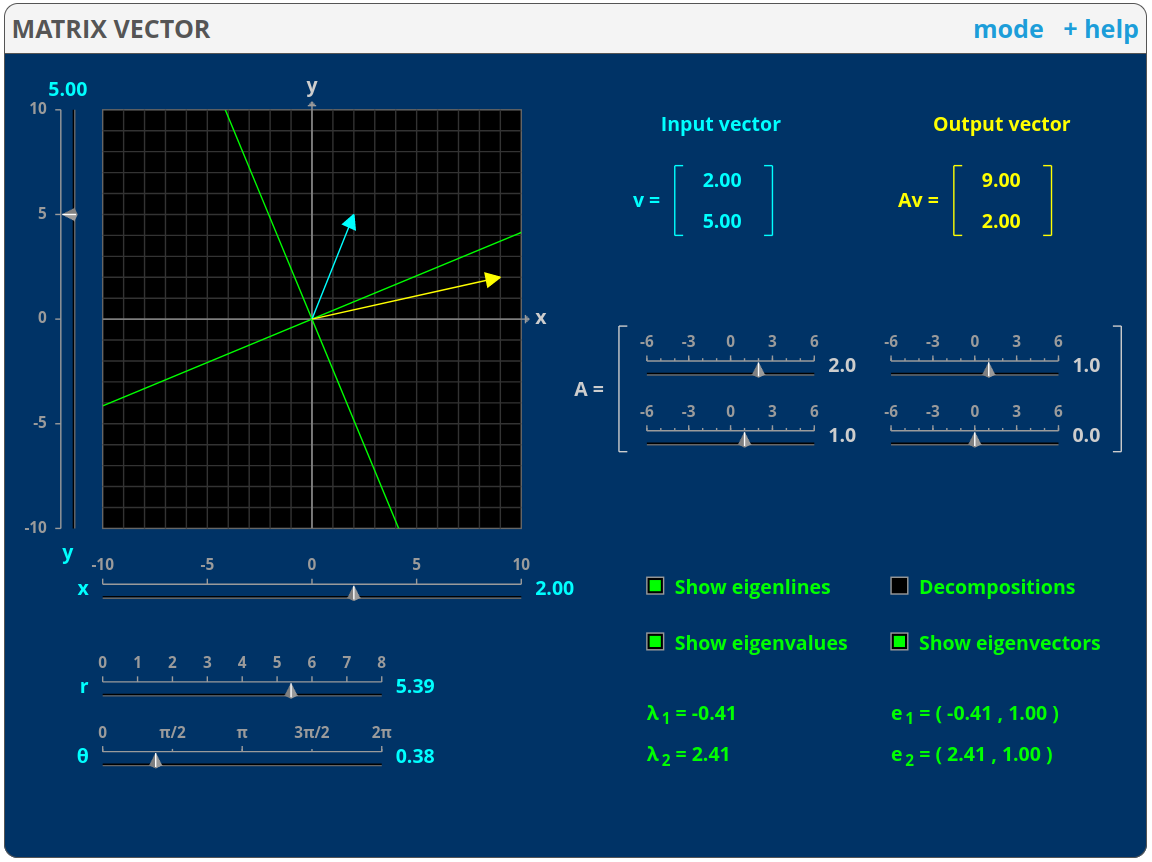
\includegraphics[width=0.85\linewidth]{mit-mathlet-matrix-vector}
	\caption{The MIT \enquote{Matrix Vector} Mathlet}
	\label{fig:mit-mathlet-matrix-vector}
\end{figure}

This app fails in two crucial ways in my opinion. It doesn't show the basis vectors or let the user drag them around, and the user can only define and therefore visualize a single matrix at once. This second problem was common among every solution I found, so I won't mention it again, but it is a big issue in my opinion and my app will allow for multiple matrices. I like the idea of having a draggable input vector and rendering its output, so I will probably have this feature in my app, but I also want the ability to define multiple matrices and be able to drag the basis vectors to visually define a matrix.

Although, in the comments on this Mathlet, a user called \enquote{David~S.~Bruce} suggested that the Mathlet should display the basis vectors, to which a user called \enquote{hrm} (who I assume to be the \enquote{H.~Miller} to whom the copyright of the whole website is accredited) replied saying that this Mathlet is primarily focussed on eigenvectors, that it is perhaps badly named, and that displaying the basis vectors \enquote{would make a good focus for a second Mathlet about 2x2 matrices}. This Mathlet does not exist. But I do like the idea of showing the eigenvectors and eigenlines, so I will definitely have that in my app.

Another web app that I found was one simply called \enquote{Linear Transformation Visualizer} by Shad~Sharma\cite{shad-io-matvis}. This one was also inspired by 3blue1brown's YouTube series. This app also has the ability to render input and output vectors and eigenlines, but it can also render the determinant parallelogram; it allows the user to drag the basis vectors; and it has the option to snap vectors to the background grid, which is quite useful. It also implements a simple form of animation where the tips of the vectors move in straight lines from where they start to where they end, and the animation is controlled by dragging a slider labelled $t$. This isn't particularly intuitive.

\begin{figure}[h]
	\centering
	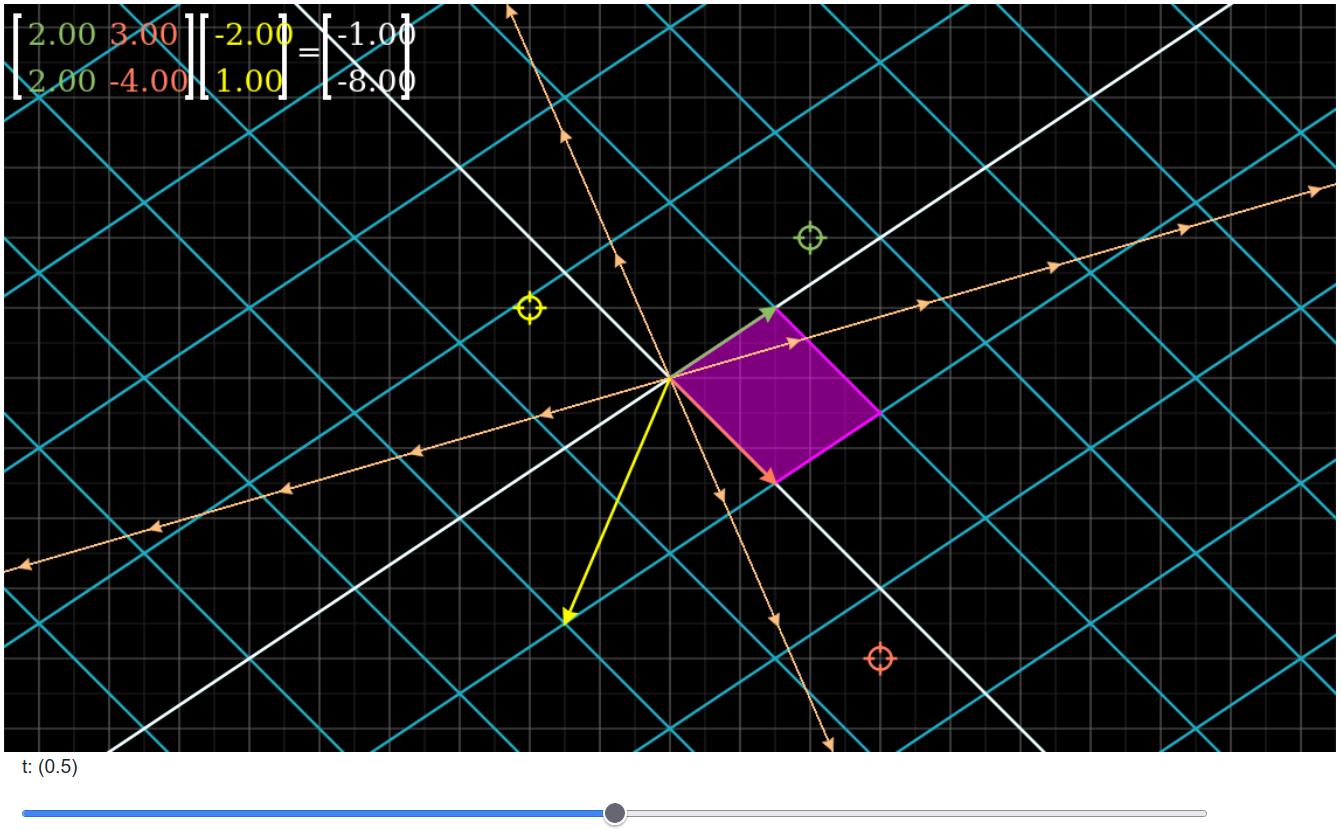
\includegraphics[width=\linewidth]{shad-io-matvis}
	\caption{Shad~Sharma's app halfway through an animation}
	\label{fig:shad-io-matvis}
\end{figure}

I really like the vectors snapping to the grid, the input and output vectors, and rendering the determinant. This app also renders positive and negative determinants in different colours, which is really nice - I intend to use that idea in my own app. However, I think that the animation system here is flawed and not very easy to use. My animation will likely be a button, which just triggers an animation, rather than a slider. I also don't like the way vector dragging is handled. If you click anywhere on the grid, then the closest vector target (the final position of the target's associated vector) snaps to that location. I think it would be more intuitive to have to drag the vector from its current location to where you want it. This was also a problem with the MIT Mathlet.

One of the solutions I found was a Desmos app\cite{desmos-2d-linear-transformation}, which was quite hard to use and arguably overcomplicated. Desmos is not designed for this kind of thing - it's designed to graph pure mathematical functions - and it shows here. However, this app brings some really interesting ideas to the table, mainly functions. This app allows you to define custom functions and view them before and after the transformation. This is achieved by treating the functions parametrically as the set of points $(t, f(t))$ and then transforming that coordinate pair by the given matrix and getting a new coordinate.
\[\begin{pmatrix}
	a & b\\
	c & d
\end{pmatrix}
\begin{pmatrix}
	t\\
	f(t)
\end{pmatrix} = \begin{pmatrix}
	at + bf(t)\\
	ct + df(t)
\end{pmatrix}\]
Desmos does this for every point and then renders the resulting transformed function parametrically. This is a really interesting technique and idea, but I'm not going to use it in my app. I don't think arbitrary functions fit with the linearity of the whole app, and I don't think it's necessary. It's just overcomplicating things, and rendering it on a widget would be tricky, because I'd have to render every point myself, possibly using something like OpenGL. It's just not worth implementing.

\begin{figure}[h]
	\centering
	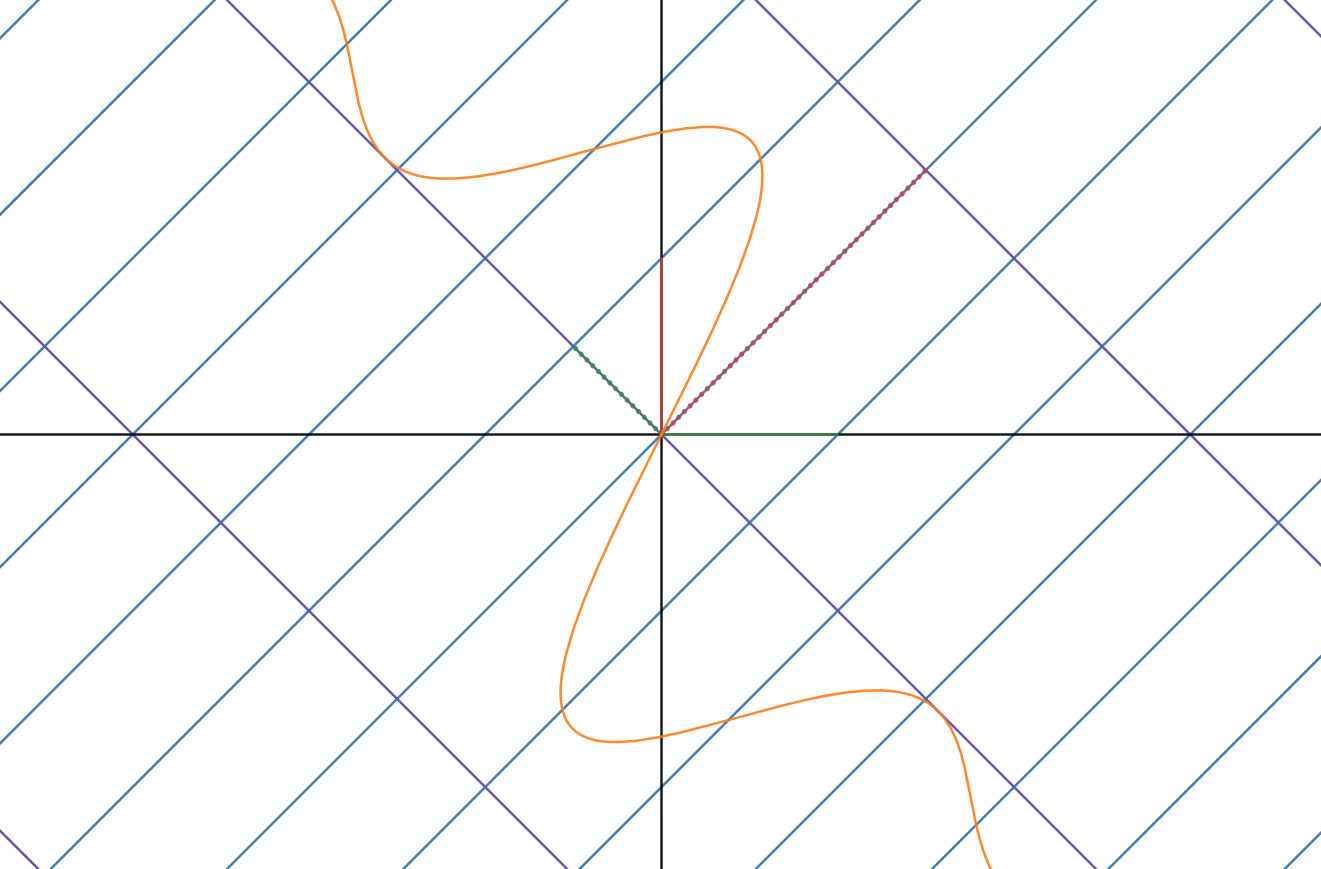
\includegraphics[width=\linewidth]{desmos-2d-linear-transformation}
	\caption{The Desmos app halfway through an animation, rendering $f(x) = \frac{\sin^2 x}{x}$ in orange}
	\label{fig:desmos-2d-linear-transformation}
\end{figure}

Additionally, this Desmos app makes things quite hard to see. It's hard to tell where any of the vectors are - they just get lost in the sea of grid lines. This image also hides some of the extra information. For instance, this image doesn't show the original function $f(x) = \frac{\sin^2 x}{x}$, only the transformed version. I will give my vectors arrowheads to make them easily identifiable.

\end{document}
